\documentclass[10pt]{article}
\usepackage{graphicx}
\usepackage{listings}
\usepackage{xcolor}
\usepackage[margin=1.8cm]{geometry}
\usepackage{tikz}

\usetikzlibrary{arrows.meta, positioning}

\setlength{\parskip}{0.4em}
\setlength{\parindent}{0pt}

\lstset{
  basicstyle=\ttfamily\small,
  keywordstyle=\color{blue},
  commentstyle=\color{gray},
  stringstyle=\color{orange},
  frame=single,
  numbers=left,
  numberstyle=\tiny, 
  breaklines=true,
  captionpos=b
}

\title{PRAC4 : Matrix Multiplication}
\author{DIETZ T., JABER A., DONNENFELD T.}
\date{\today}

\begin{document}

\maketitle

\section{Step 1: Theoretical Analysis}

\subsection{Iterative Version: Work Partitioning}

For the classical iterative matrix multiplication, we parallelize the computation
by distributing the \textbf{rows of the output matrix} across the available threads.
Matrix multiplication has no data dependencies between rows of $C$ because:

\[
C[i,j] = \sum_{k=0}^{N-1} A[i,k]\,B[k,j],
\]


With $k$ threads, we partition rows of C into $k$ blocks

Each thread:
\begin{itemize}
    \item reads $\frac{N}{k}$ rows of $A$,
    \item reads all of $B$,
    \item writes to disjoint rows of $C$.
\end{itemize}

This gives perfect load balance if matrix has data evenly distributed across its rows and columns and no race conditions.

In particular for two threads:

\includegraphics[scale=0.40]{../out/matmul_2_threads_schema.jpeg}

\subsection{Divide and Conquer Version}

The recursive version repeatedly divides the problem into 8 independent
subproblems of size $\frac{SZ}{2}\times \frac{SZ}{2}$ until the base-case size
$DQSZ$ is reached.

By analogy with the same 1 dimension problem : we find the number of required splits steps $n$ = $\log_2\!\left(\frac{N}{DQSZ}\right)$ 


At recursion level $i$, the number of tasks is 8^{\,i}

The total number of tasks is the sum of the terms of the previous geometric sequence, n being the max number of splits seen above.
Therefore : 
T = \sum_{i=1}^{n} 8^{\,i}
  = \frac{8^{\,n+1} - 8}{7}.


The maximum concurrency is the number of "leaf" tasks when all tasks have been created: 8^{\,s}

\subsubsection*{Case for $N=1024$, $DQSZ=512$}

Here $s = \log_2(1024/512)=1$, so only one level of recursion.

\begin{center}
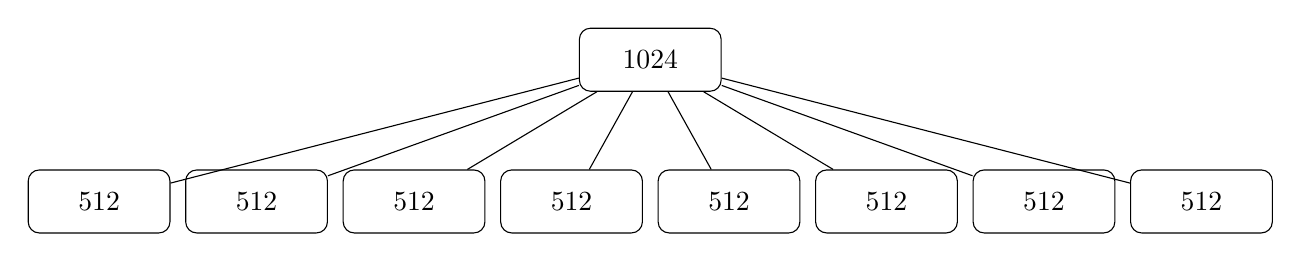
\begin{tikzpicture}[
  task/.style={rectangle,draw,rounded corners,align=center,minimum width=1.8cm,minimum height=0.8cm},
  level distance=1.8cm,
  sibling distance=2cm
]

\node[task] (root) {1024}
child { node[task]{512} }
child { node[task]{512} }
child { node[task]{512} }
child { node[task]{512} }
child { node[task]{512} }
child { node[task]{512} }
child { node[task]{512} }
child { node[task]{512} };

\end{tikzpicture}
\end{center}



\[
s = 1,
\qquad
T = 8,
\qquad
\text{Max concurrency} = 8.
\]

\subsubsection*{Memory Access per Task}

We have to be careful with the tasks : sums and products of $A$ and $B$ submatrices can run in parallel,
but these results have to be added two by two to form submatrices of $C$ : this causes values in $C$ to be accessed by two tasks possibly at the same time. 

\section{Step 2: Practical Parallel Implementation}

\subsection{Iterative Version}

We unroll the loops to take advantage of contiguous memory operations and potential SIMD vectorization.

\begin{lstlisting}[language=C++]
#pragma omp parallel for
for (int i=0; i<N; i+=2)
  for (int k=0; k<N; k+=2)
    for (int j=0; j<N; j++)
    {
      type B1 = b[k*N+j];
      type B2 = b[(k+1)*N+j];

      c[i*N+j]     += a[i*N+k]     *B1 + a[i*N+k+1]     *B2;
      c[(i+1)*N+j] += a[(i+1)*N+k] *B1 + a[(i+1)*N+k+1] *B2;
    }
\end{lstlisting}

This reduces memory accesses.

\subsection{Divide and Conquer Version}

We parallelize the recursion using OpenMP tasks:

\begin{lstlisting}[language=C++]
#pragma omp parallel
{
  #pragma omp single
  {
    #pragma omp task { ... }
    #pragma omp task { ... }
    #pragma omp task { ... }
    #pragma omp task { ... }
  }
}
\end{lstlisting}

\section{Step 3: Performance Analysis}

We benchmarked $N=2048$ for a range of thread counts and $DQSZ$ values.  
Counters collected using \texttt{perf stat}:

\begin{itemize}
    \item execution time,
    \item instructions, cycles, IPC,
    \item cache misses,
    \item speedup and efficiency.
\end{itemize}

\subsection{Heatmap 1: Execution Time}

\begin{center}
  \includegraphics[width=0.55\linewidth]{../out/duration_time_heatmap_log_all.pdf}
\end{center}

Observations:
\begin{itemize}
    \item Large and very small $DQSZ$ (4, 8, 2048) yields very poor performance
    \item Single threaded runs yield very poor performance
    \item $DQSZ=64$ or $DQSZ=128$ produce the best runtimes.
    \item There seem to be a special increase in performance if the number of thread is a multiple of 4
          (looking at nb threads=6 in the graph)
\end{itemize}

This graph shows the overall best configurations for this problem on the machine.

\subsection{Heatmap 2: Speedup (vs same-$DQSZ$, single-thread)}

\begin{center}
  \includegraphics[width=0.55\linewidth]{../out/speedup_heatmap.pdf}
\end{center}

Interpretation:

\begin{itemize}
    \item Speedup is highest for small base-case sizes (8 and 16).
    \item Large $DQSZ$ values generate too few tasks, limiting parallelism.
    \item Small $DQSZ$ values enable enough fine-grained tasks to keep all
    threads busy.
\end{itemize}

This graph explains that for some DQSZ we take much more advantage of parallelism,
but doesn't prove that global execution time is better ( memory bandwidth limitations). 

\subsection{Heatmap 3: Cache Misses per Instruction}

\begin{center}
  \includegraphics[width=0.55\linewidth]{../out/cachemiss_perinst_heatmap.pdf}
\end{center}

Interpretation :

\begin{itemize}
    \item Cache misses per instruction are minimal for $DQSZ=8$ and $DQSZ=16$.
    \item Their working sets fit inside caches ( L1/L2 ?)
    \item Larger $DQSZ$ values overflow L1/L2 and drastically increase miss rate.
\end{itemize}

We find a sweet spot of DQSZ=16 for cache optimization,
probably related to the size of the L1 cache compared to the DQSZ size in memory.

\end{document}
